% !TEX root = main.tex

\section{代码生成及优化}
\subsection{代码生成}
\begin{itemize}
	\item 指令选择:选择最适合目标机器的指令来实现IR
	\item 寄存器分配和指派
	\item 指令调度
\end{itemize}

\begin{definition}[基本块(basic block)]
单一入口单一出口。
成为leader的指令:
\begin{enumerate}
	\item 第一条三地址指令
	\item 条件或无条件跳转指令的目标
	\item 条件或无条件跳转指令的下一指令
\end{enumerate}
\end{definition}

\begin{example}
考虑以下基本块:
\[\begin{aligned}
t_0 &= 5\\
t_1 &= 3 * t_0\\
t_2 &= R + r\\
t_3 &= t_1 * t_2\\
t_4 &= t_2\\
t_5 &= t_3 - t_4\\
t_6 &= t_1 * t_2\\
A   &= t_6 + t_5\\
B   &= A - r\\
t_7 &= t_1\\
B   &= t_7 + B
\end{aligned}\]
\begin{enumerate}
\item 构造这一基本块的DAG.
\item 假设只有$A$和$B$在基本块后面还要被引用,产生优化后的三地址代码.
\end{enumerate}
\end{example}
\begin{analysis}
\begin{enumerate}
	\item 基本块的DAG如下图所示
	\begin{figure}[H]
	\centering
	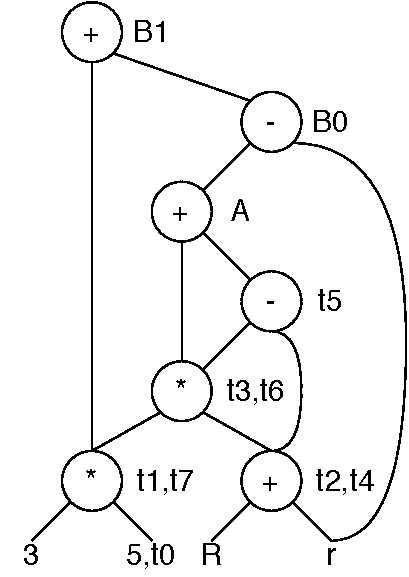
\includegraphics[width=0.3\linewidth]{fig/dag-1.pdf}
	\end{figure}
	\item 由于只有$A$和$B$在基本块后面还要被引用,因此最终只需保留$A$和$B$的结果即可。
	无依赖关系的代码都可以作为死代码优化删除。
	最终优化后的三地址代码如下
\[\begin{aligned}
t_2 &= R + r\\
t_3 &= 15 * t_2\\
t_5 &= t_3 - t_2\\
A &= t_3 + t_5\\
B &= A - r\\
B &= 15 + B
\end{aligned}\]
\end{enumerate}
\end{analysis}

\subsection{代码优化}
\begin{itemize}
	\item 窥孔优化(peephole):基于滑动窗口,最小粒度
\begin{lstlisting}[language=c++]
x = x + 0 // eliminated
x = x * 1 // eliminated
y = x * 2 // y = x << 1
LD R0, a
ST a, R0 // eliminated
\end{lstlisting}
	\item 局部优化:在基本块内的优化
\begin{itemize}
	\item 公共子表达式删除
	\item 常量/拷贝传递
	\item 冗余操作消除
\end{itemize}
	\item 循环优化:在循环内的优化
	\item 全局优化:最粗粒度的优化
\end{itemize}

\begin{definition}[循环(loop)]
只有唯一入口/头的强连通子图
\end{definition}

\begin{example}
考虑下列代码片段:
\begin{enumerate}[label=(\arabic*)]
\item \verb'm := 0'
\item \verb'v := 0'
\item \verb'if v >= n goto (19)'
\item \verb'r := v'
\item \verb's := 0'
\item \verb'if r < n goto (9)'
\item \verb'v := v + 1'
\item \verb'goto (3)'
\item \verb's := v + r'
\item \verb'y := 0 * x'
\item \verb'z := v - y'
\item \verb'x := z + r'
\item \verb'r := m - x'
\item \verb'if s <= m goto (17)'
\item \verb'm := s'
\item \verb's := s + r'
\item \verb'r := r+1'
\item \verb'goto (6)'
\item \verb'return m'
\end{enumerate}
为这段代码划分基本块(Basic Block),并画出控制流图(Control Flow Graph).
在答案中你可以直接画出控制流图,但对图中的每个结点,请用$m\thicksim n$表示相应的基本块由第$m$至第$n$条语句组成.
\end{example}
\begin{analysis}
如下图所示,共$9$个基本块,每个基本块包含的语句已在图中标出。
\begin{figure}[H]
\centering
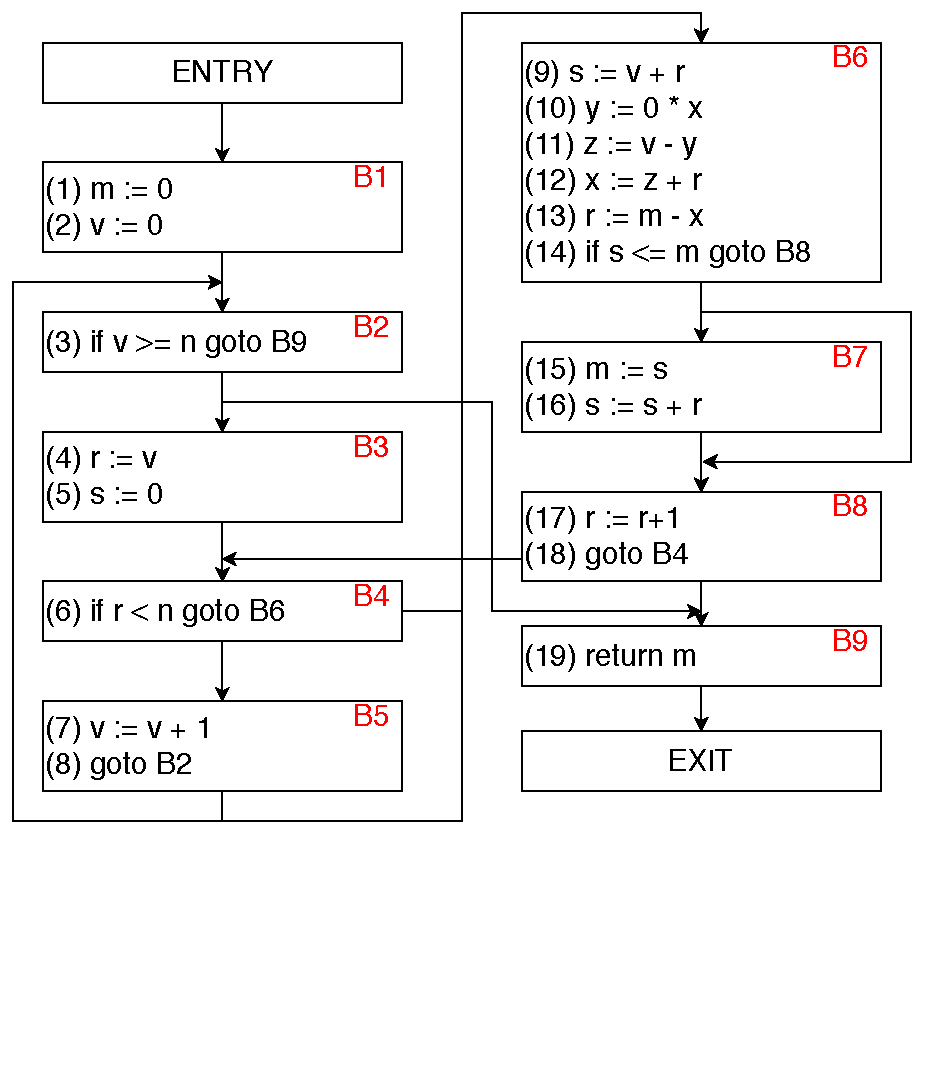
\includegraphics[width=0.7\linewidth]{fig/dag-2.pdf}
\end{figure}
\end{analysis}